\documentclass[11pt, class=article, crop=false]{standalone}
\usepackage[subpreambles=true]{standalone}
\usepackage{newtxtext,newtxmath}
\usepackage{import,
            graphicx,
            parskip,
            url,
            amsmath,
            wrapfig,
            fancyhdr,
            soul,
            tabularx,
            authblk,
            textcomp,
            lineno,
            setspace}

% side caption figure
\usepackage{sidecap}
\sidecaptionvpos{figure}{t}

% for special characters in bibliography            
\usepackage[utf8]{inputenc}
\usepackage[T1]{fontenc}

% citation setup
\usepackage[euler]{textgreek}
\usepackage[numbers,sort&compress]{natbib}
\setcitestyle{square, comma}
\bibliographystyle{vancouver} % for prceedings B (Royal society publishing)

% caption setup
\usepackage[font = small, labelfont = {bf, small}]{caption}
           
% margin
\usepackage[top=2.54cm, bottom=2.54cm, left=2.54cm, right=2.54cm]{geometry}

\linenumbers
\doublespacing

% title
%\title{Body size and local density influence movement patterns in stream fish}
\date{} % remove date from title

% author list
%\author{} % remove author list from main text 

%\maketitle
% title
\title{Body size and local density explain movement patterns in stream fish}
\date{} % remove date from title

% author list
\author[1]{Ashley LaRoque}
\author[1, 2]{Seoghyun Kim}
\author[1]{Akira Terui}
\affil[1]{Depatment of Biology, University of North Carolina at Greensboro}
\affil[2]{Department of Biological Sciences, Kangwon National University}

\begin{document}

\maketitle
\thispagestyle{empty}

\section*{Contact}
Akira Terui by email at \url{a_terui@uncg.edu}

\newpage
\thispagestyle{empty}

\section*{Keywords}

fish movement, body size, density-dependent, movement drivers, extrinsic and intrinsic, freshwater

\section*{Abstract}

 Movement is a fundamental process in structuring communities, distributing species, and mediating gene flow. Both extrinsic (e.g., density of species) and intrinsic factors (e.g., body size) influence movement patterns, ultimately driving the spatial organization of ecological communities. However, these extrinsic and intrinsic factors are often assessed in isolation, limiting our ability to understand how multiple factors combine to shape movement patterns in nature. Here, we evaluate whether body size (intrinsic) and intra- and interspecific densities (extrinsic) have an impact on the movement rates of four fish species (\textit{Nocomis leptocephalus} bluehead chub, \textit{Semotilus atromaculatus} creek chub, \textit{Lepomis cyanellus} green sunfish, and \textit{L. auritus} redbreast sunfish) in a small stream. We employed a capture-mark-recapture framework to individually track movements, defined as the difference between locations on consecutive (re)captures. We then applied a dispersal-observation model that accounts for detectability, survival, and emigration when inferring movement processes. We found that larger individuals of creek chub and green sunfish were more likely to move, which may be explained by their greater physical ability to balance the energetic cost of moving in tandem with greater competitive ability during settlement. The effect of density on movement was mixed, such that both green and redbreast sunfish responded to creek chub positively, but conversely to the bluehead chub. Collectively, our results suggest that intrinsic (body size) and extrinsic factors (density) influence movement patterns, but their relative importance is species-specific. Further exploring the mechanistic relationship behind drivers of movement will provide greater insight into spatial community dynamics.

\clearpage
\pagenumbering{arabic} 
\newpage

\section{Introduction}

Movement is a ubiquitous characteristic of animals, mediating nutrient exchange, gene flow, and disease spread, among others \citep{cookeMovementEcologyFishes2022, hessDiseaseMetapopulationModels1996, teruiParasiteInfectionInduces2017, fauschLandscapesRiverscapesBridging2002}.
If successful, movers may obtain substantial benefits such as release from intense competition and disease risks \citep{clobertDispersalEcologyEvolution2012, teruiParasiteInfectionInduces2017}.
However, it comes with energetic and opportunity costs \citep{bonteCostsDispersal2012}.
Mobile individuals must make an appropriate decision on when and how they move to improve their fitness, such as growth and survival \citep{bonteCostsDispersal2012}. As a result, movement is influenced by both extrinsic and intrinsic factors with important consequences for spatially-structured communities \citep{leiboldMetacommunityConceptFramework2004, mcpeekEvolutionPassiveDispersal2024, schlagelMovementmediatedCommunityAssembly2020}. 

Body size exemplifies intrinsic individual conditions that affect movement patterns \citep{clobertDispersalEcologyEvolution2012}. For example,  larger individuals tend to move long distances due in part to their greater locomotive capabilities, although the nature of correlation varies greatly among species and ecological contexts \citep{comteEvidenceDispersalSyndromes2018, teruiParasiteInfectionInduces2017, radingerPatternsPredictorsFish2014, debeffeConditiondependentNatalDispersal2012,gilliamMovementCorridorsEnhancement2001}.
Simultaneously, intra- and interspecific population densities -- key extrinsic factors -- influence movement through competitive and mutualistic interactions. For example, competitive interactions may cause individuals to move away from densely populated areas, while mutualistic interactions and higher prey availability may reduce movement rates \citep{thierryInterplayAbioticBiotic2024, rasmussenIndividualMovementStream2017, fronhoferBottomupTopdownControl2018}.

Despite this recognition, the interplay between extrinsic and intrinsic factors on movement has rarely been considered. Most previous studies have evaluated these factors in isolation due to field constraints and statistical complexity. However, this makes it difficult to understand how movement patterns may persist in nature because these drivers lack mutual exclusivity \citep{mcmahonLinkingHabitatSelection2006}. 
This unified perspective is particularly important, yet challenging to implement in the field, where multiple species interact and may exhibit species-specific responses to both intrinsic and extrinsic factors \citep{teruiNonrandomDispersalSympatric2021}. Addressing this complexity in movement ecology requires a tractable system, where one can directly observe movement processes while maintaining relevance to natural communities.

Here, we aim to evaluate movement patterns of stream fishes in response to an extrinsic (population density) and intrinsic driver (body size) because they serve as an excellent model system. In a small stream, their movement is restricted to a one-dimensional system (either up- or downstream movement), making the direct observation of movement processes highly tractable in the wild. In addition, as individuals of various sizes move across habitat patches, they engage in inter- and intraspecific interactions over space and time \citep{brownHabitatHeterogeneityActivity2010, davidsonSeasonalSpatialHydrological2012, robinsonEffectsMultiyearExperimental2003, albaneseEcologicalCorrelatesFish2004, nakayamaFinescaleMovementEcology2018, pettyRestrictedMovementMottled2004, robertsSpatiotemporalVariabilityStream2007}.
We used a mark-recapture framework conducted seasonally over a four-year period to model movement responses while considering survival, detectability, and emigration. 
We hypothesize that both intrinsic and extrinsic factors influence the movement of stream fishes.
Specifically, we tested the following predictions:  (1) larger individuals move more often than their smaller counterparts; (2) higher interspecific densities will drive more movement due to competition; and (3) higher intraspecific density will drive more movement among conspecifics.

\section{Method}

\subsection{Study Site and Species}

Our study was conducted in a small tributary of the Reedy Fork River ($\sim$3 m in wet width), located in the Piedmont region of North Carolina, USA (36$^\circ$16’99.39”N, 79$^\circ$72’20.88”W). 
This stream consisted of riffle-pool sequences with its substrate dominated by sand and gravel.
At base-flow conditions, the average wetted width is $\sim$3 m with a mean depth of $\sim$0.2 m. 

We selected a 430-m reach of the stream for our mark-recapture research. Among water-column species, four species dominated in the study reach (85\% in cumulative abundance): two cyprinids (\textit{Nocomis leptocephalus} bluehead chub  (38\% in abundance) and \textit{Semotilus atromaculatus} creek chub (19\% in abundance)) and two centrarchids (\textit{Lepomis cyanellus} green sunfish (19\% in abundance) and \textit{L. auritus} redbreast sunfish (9\% in abundance)). All four species are known to exhibit resident (non-migratory) life-history strategies \citep{teruiNonrandomDispersalSympatric2021}. Other water-column and benthic species found (ordered from common to rare) within this reach include: \textit{Etheostoma olmstedi} tessellated darter, \textit{Moxostoma rupiscartes} striped jumprock, \textit{L. macrochirus} bluegill, \textit{Micropterus salmoides} largemouth bass, \textit{Noturus insignis} margined madtom, \textit{Fundulus rathbuni} speckled killifish, \textit{M. collapsum} notchlip redhorse, \textit{Luxilus albeolus} white shiner, \textit{Erimyzon oblongus} creek chubsucker, \textit{Gambusia holbrooki} eastern mosquitofish, \textit{Misgurnus anguillicaudatus} pond loach, \textit{L. gulosus} warmouth, \textit{Clinostomus funduloides} rosy side dace, and \textit{Ameiurus natalis} yellow bullhead. 

\subsection{Fish Sampling}

We focused on the dominant fish species in the study reach for our mark-recapture study. Mark-recapture sampling took place regularly from November 2020 to August 2024 at an interval of roughly three months (average 93 days), except for one interval (November 2021 to May 2022; 171 days) in which we were unable to conduct a field survey in February 2022 for logistical reasons. As a result, we collected mark-recapture data for 15 occasions.

The study reach was divided into 10-m sections to locate fish at a fine spatial scale. In each section, fish were collected via single-pass electrofishing (Smith-Root, Inc.) and placed in a five-gallon bucket for handling. All captured individuals were identified to species and measured for total length (mm). Individuals of the study species (> 60 mm in total length) were anesthetized with MS-222 (Tricaine-S) and implanted with a 12-mm passive integrated transponder (PIT) tag to uniquely identify each individual in subsequent recaptures (Oregon RFID). This technique has been described in more detail by Cary et al. (2017). These individuals were also weighed (g). A liquid skin glue was used on the incision site for individuals of both chub species to prevent tag loss due to the nature of their scales. After the successful implantation, fish were returned to their holding bucket and monitored to ensure survival before being released back into their section of capture. 

\subsection{Environmental Variables}

Habitat variables were measured at base-flow conditions along three evenly spaced transects per section. In each transect, we measured the following physical variables at the center and near both sides of the bank, totaling nine measurements per section: water depth (nearest cm), current velocity (m/s), and dominant substrate type (silt, <0.1 mm; sand, 0.1--2 mm; gravel, 2--16 mm; pebble, 16--64 mm; cobble, 64--256 mm; boulder, 256--512 mm; bedrock, >512 mm). In addition, we measured the total aerial coverage of habitat refuge areas (HRA; m$^2$) like undercut banks and woody debris per section as these structures may represent important microhabitats for the study species. We approximated the areal coverage as the area of the rectangular, calculated as the length times the mean width measured at the three points of the structure.

We calculated the surface area of each section as the mean wet width (measured at each transect) times the section length. Water temperature and pressure were monitored hourly using a water level logger (HOBO® Onset, Model U20L-02) deployed at the upstream end of the study reach.

\subsection{Statistical Analysis}

We used the dispersal-observation model to evaluate the effects of both intrinsic and extrinsic variables on movement behaviors \citep{teruiModelingDispersalUsing2020, teruiNonrandomDispersalSympatric2021, teruiParasiteInfectionInduces2017, rodriguezRestrictedMovementStream2002}. This modeling approach fundamentally differs from ordinary linear models (e.g., generalized linear models) in two key ways. First, it integrates movement and observation processes into a single model. In field studies, observed movement is often confounded by imperfect detection and unmeasured emigration or mortality. The dispersal-observation model yields less biased estimates of movement parameters by explicitly accounting for these factors \citep{teruiModelingDispersalUsing2020}. Second, this framework models the \textit{dispersion} parameter of the movement kernel, i.e., the spread of movement distances, as a function of linear predictors. This contrasts with conventional linear models, which typically relate predictors to the \textit{mean} of a distribution. As a result, this approach more appropriately captures variation in movement behavior across ecological contexts \citep{teruiModelingDispersalUsing2020, pepinoFishDispersalFragmented2012, rodriguezRestrictedMovementStream2002}.

\textit{Movement process}. We define movement as fine-scale shifts over habitat patches that occur between consecutive recapture events (i.e., movement between occasion $t$ and $t+1$). Let $X_{1,i}$ and $X_{0,i}$ denote locations of recapture at occasion $t+1$ and capture at occasion $t$ for individual replicate $i$, which were measured as the distance from the midpoint of the section to the downstream end of the study stretch. We assumed $X_{1,i}$ as a random draw from a Student-t distribution conditional on the capture location $X_{0,i}$ as:    

\begin{equation}
    X_{1, i}|X_{0, i}, \sigma_i \sim \text{t}(X_{0, i}, \sigma_i^2, \nu)
    \label{eq:student-t}
\end{equation}

where $\sigma_i$ is the standard deviation describing the distance moved between consecutive capture and recapture occasions ($X_{1,i} - X_{0,i}$), and $\nu$ is the degree of freedom.
We chose a Student-t distribution because movement data are often heavy-tailed \citep{clobertDispersalEcologyEvolution2012}.
The degrees of freedom parameter, $\nu$, controls the extent of heavy-tailedness, with lower values indicating fatter tails. As $\nu$ approaches infinity, the Student-t distribution converges to a normal distribution.
Using a Student-t distribution allows us to draw robust inferences about the ecological drivers of movement by properly accounting for outliers; i.e., the coefficient estimates remain relatively insensitive to them (see Equation \ref{eq:linear-pred}) \citep{lunnBUGSBookPractical2012}.

We linked the standard deviation of  movement distance to predictors using a log-link function: 

\begin{equation}
    \ln \sigma_i = \beta_0 + \sum_{k} \beta_k x_{k,i} + \ln \eta_i
    \label{eq:linear-pred}
\end{equation}

where $\beta_0$ is the intercept and $\beta_k$ is the regression coefficient for the $k$-th predictor $x_{k,i}$. The log-transformed time interval between capture and recapture $\ln \eta_i$ [ln day] was included as an offset term to standardize the movement duration between observations.

Our model included the following predictors ($x_k$ in Equation \ref{eq:linear-pred}): body size, weighted densities of dominant fish species (bluehead chub, creek chub, green sunfish, and redbreast sunfish), mean water temperature, HRA, and current velocity.
We included body size at capture as a proxy variable for the individual’s locomotive capacity (internal factor), whereas the weighted fish densities were included to evaluate intra- and interspecific density-dependence in movement (external factors).
Fish densities were weighted by distance to the capture location to reflect that fish individuals in close proximity may have a greater influence on movement.
Specifically, the distance-weighted fish density at section $s$, denoted $D^{(w)}_s$, was calculated as $D^{(w)}_s = \sum_{s'} D_{s'}\exp(-\lambda d_{ss'})$, where $D_{s'}$ is the fish density corrected for season-specific imperfect detection (see SI, Detection Model and Table S1), $d_{ss'}$ is the separation distance between the midpoints of sections $s$ and $s'$, and $\lambda$ is a rate parameter that defines how quickly the density weight decays with increasing separation distance. 
We set $\lambda = 0.1$, indicating that density influences are strongest within approximately 10 meters, while still allowing for non-negligible contributions from greater distances.
We chose this value because previous studies have consistently shown that stream fishes typically remain within 10–20 meters over extended periods, although some individuals do disperse over longer distances \citep{skalskiModelingDiffusiveSpread2000, pepinoFishDispersalFragmented2012, rodriguezRestrictedMovementStream2002, teruiNonrandomDispersalSympatric2021, radingerPatternsPredictorsFish2014}.

In our model, mean water temperature (averaged over each sampling interval) was included to account for potential seasonality in movement patterns, and HRA and current velocity were incorporated to control for possible effects of microhabitat structure variation between sections. HRAs often provide microhabitats that harbor a considerable number of individuals. Other habitat variables, such as depth and substrate, were not included due to their correlation with velocity. The inclusion of these predictors allows the model to evaluate the effects of body size and fish densities after accounting for potential influences of confounding factors.

\textit{Observation process}. Our capture-recapture data is the imperfect representation of movement processes because fish are recaptured only when the following conditions are satisfied simultaneously: alive, stay, and detected in the study section. Our observation model accounts for this process by describing the recapture state $Y_i$ (1 if recaptured 0 otherwise) as random draws from a Bernoulli distribution:

\begin{equation}
    Y_i \sim \text{Bernoulli}(\phi z_i)
\end{equation}

where $\phi$ is the product of survival, detection, and tag-retention probabilities (hereafter, ``recapture'' probability) and $z_i$ is the binary latent variable indicating whether individual $i$ stayed in the study section at the recapture occasion.
The latent variable $z_i$ was determined by the observed (if recaptured) or predicted location (if not recaptured) of individual replicate $i$ as: 

\begin{equation}
    z_i =
    \begin{cases}
        1~\text{if}~0 \le X_{1,i} \le L~\text{(stay)},\\
        0~\text{otherwise (emigrate)}.
    \end{cases}
\end{equation}

$L$ is the upstream terminal of the study reach ($L = 430$). When $X_{1,i}$ was unobserved (i.e., not recaptured), a predicted value was drawn from Equation \ref{eq:student-t} through the Markov Chain Monte Carlo simulations (see below), thus accounting for the observation process when estimating the movement parameter $\sigma_i$.
This coupling of observation and movement processes accounts for permanent emigration and yields less biased estimates of movement parameters \citep{teruiModelingDispersalUsing2020}.

The model was fitted to the data for each species separately using JAGS \citep{plummerJAGSProgramAnalysis2003}. Weakly informative priors were assigned to parameters: $\text{Normal}(0, 2.5^2)$ for intercept $\beta_0$, $\text{Normal}(0, 1^2)$ for coefficients $\beta_k$, $\text{Trunc}(\text{Normal}(0.5, 1^2), 0, 1)$ for recapture probability $\phi$, and $\text{Trunc}(\text{Exp}(0.1), 3, \infty)$ for the degree of freedom $\nu$. Markov chain Monte Carlo (MCMC) simulations were run for 45,000 iterations with a 15,000 burn-in period and we retained 1,000 samples per chain by thinning every 30 steps to calculate posterior probabilities. Model convergence was checked by ensuring that the potential scale reduction factor, referred to as R-hat, was less than 1.1 for all parameters. All statistical analyses were conducted in R version 4.4.0 \citep{rcoreteamLanguageEnvironmentStatistical2021}.

\section{Results}

Across 15 sampling occasions, we tagged 2,430 unique individuals of our target species, 273 of which were recaptured at least once in consecutive surveys (SI, Table S2).  
Absolute movement distances ranged from 0 to 390 m across species and seasons.  
For tagged individuals, redbreast sunfish exhibited the largest mean body size ($96.2 \pm 24.4$ mm), followed by creek chub ($92.4 \pm 21.1$ mm), bluehead chub ($91.4 \pm 21.0$ mm), and green sunfish ($84.6 \pm 18.4$ mm) (SI, Table S3).
Creek chub was the most abundant species ($0.62 \pm 0.55$ individuals/m$^2$), followed by green sunfish ($0.51 \pm 0.50$), bluehead chub ($0.30 \pm 0.32$), and redbreast sunfish ($0.29 \pm 0.48$) (SI, Table S4).  

\begin{figure}
    \centering
    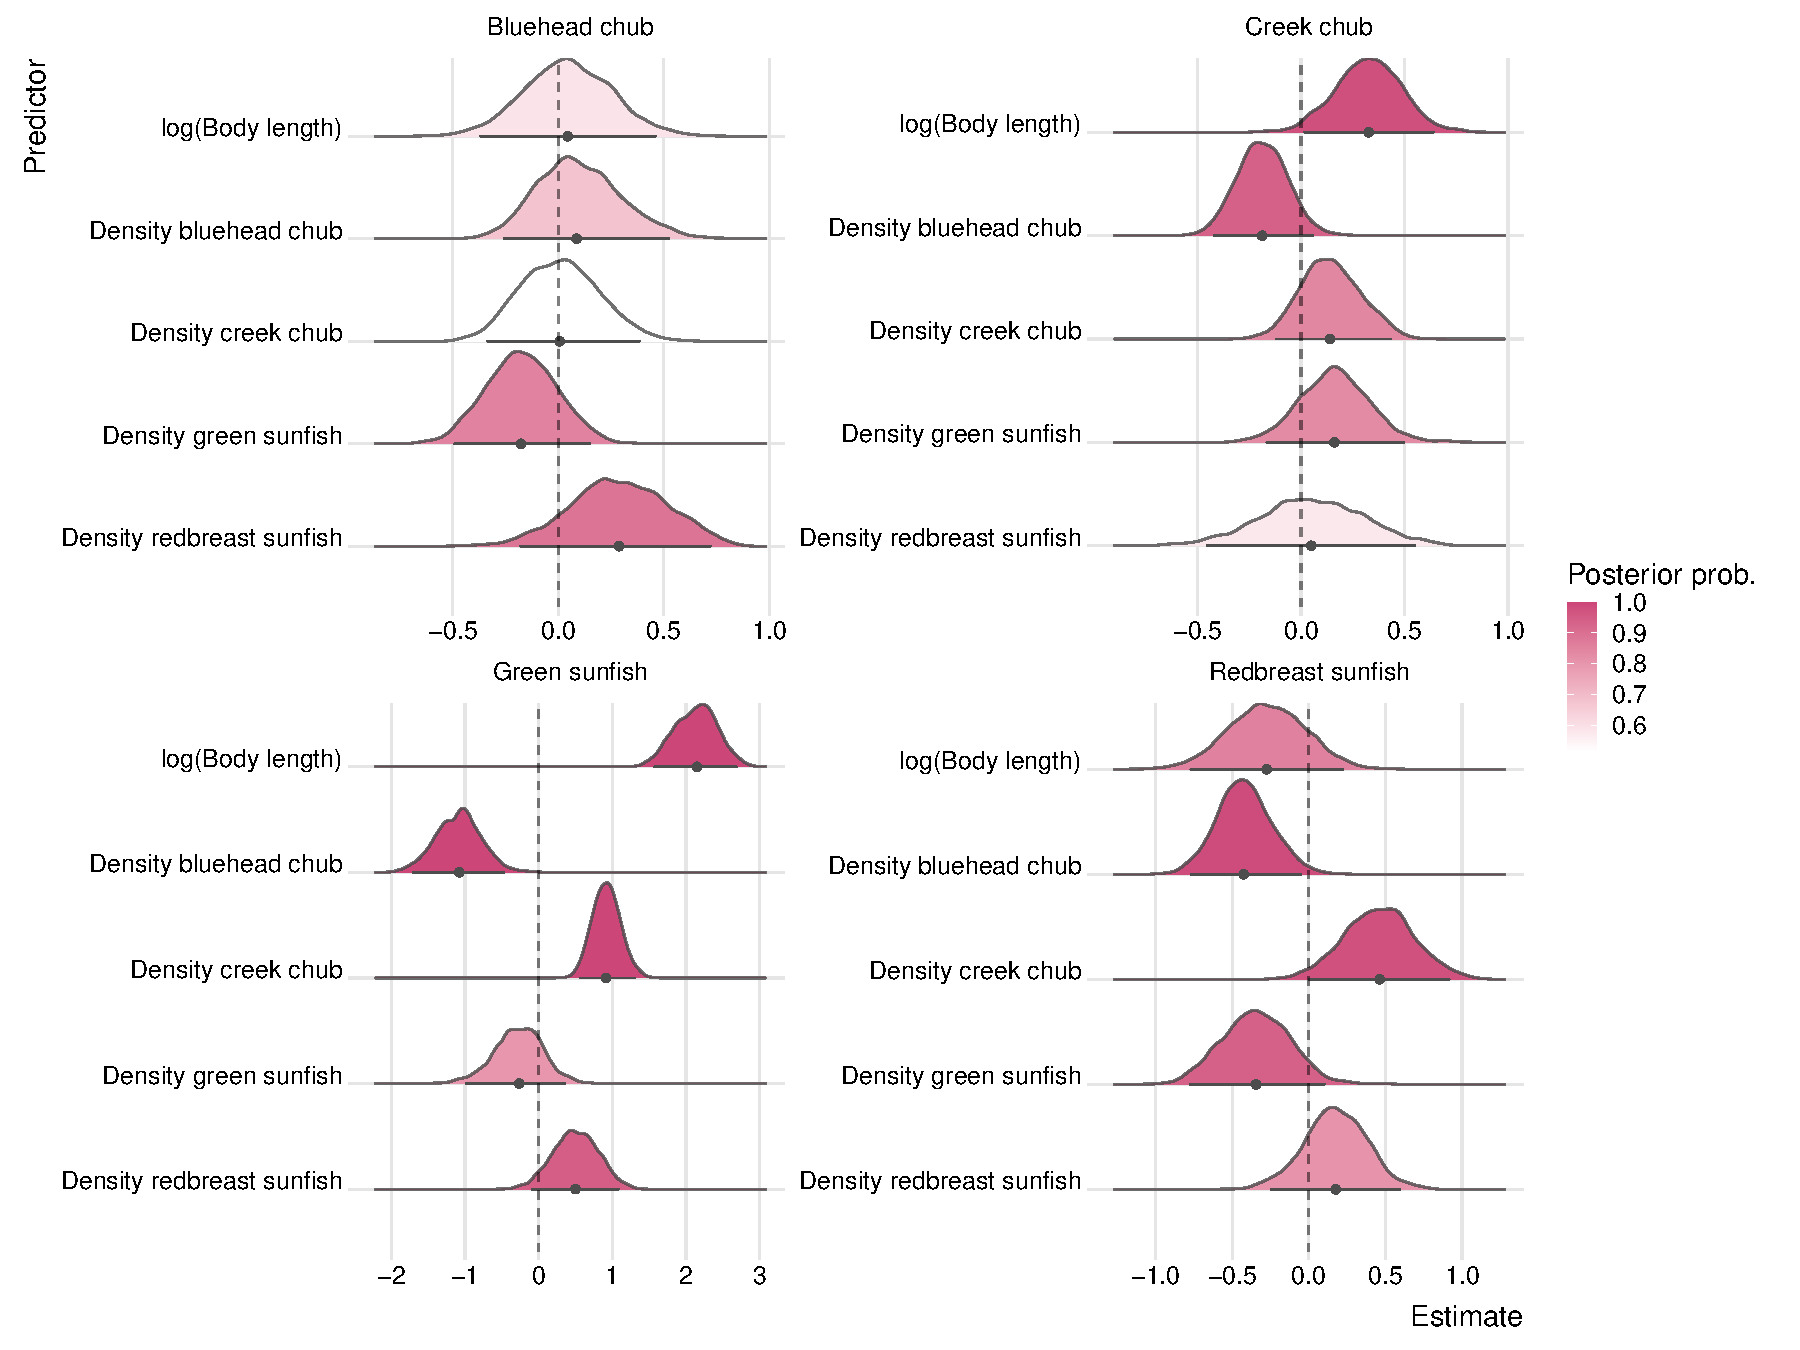
\includegraphics[width=0.9\linewidth]{output/fig_est.pdf}
    \caption{Posterior distributions for parameters in the dispersal-observation model. Median estimates are denoted by points with error bars showing the traditional 95\% credible interval. 
    Distributions are colored in proportion to the posterior probability of each parameter (approximated as the proportion of MCMC samples above or below zeros).
    Higher values of the posterior probability indicate statistically robust effects.
    Note that our model also included mean water temperature, habitat refuge area, and current velocity to minimize potential bias in estimating the effects of body size and fish densities.
    Full parameter estimates are provided in Table S5.}
    \label{fig:fig_est}
\end{figure}

Our model analysis revealed that movement responses to body size and density are highly species-specific (Figure \ref{fig:fig_est}). Creek chub and green sunfish increased movement distance with their body size, and their posterior probabilities were greater than 0.95 (Figures \ref{fig:fig_est} and \ref{fig:fig_size}; see also Table S5). 
However, the movement patterns of bluehad chub and redbreast sunfish showed vague relationships with body size, with the posterior distributions centered around zero (Figure \ref{fig:fig_est}).

\begin{figure}
    \centering
    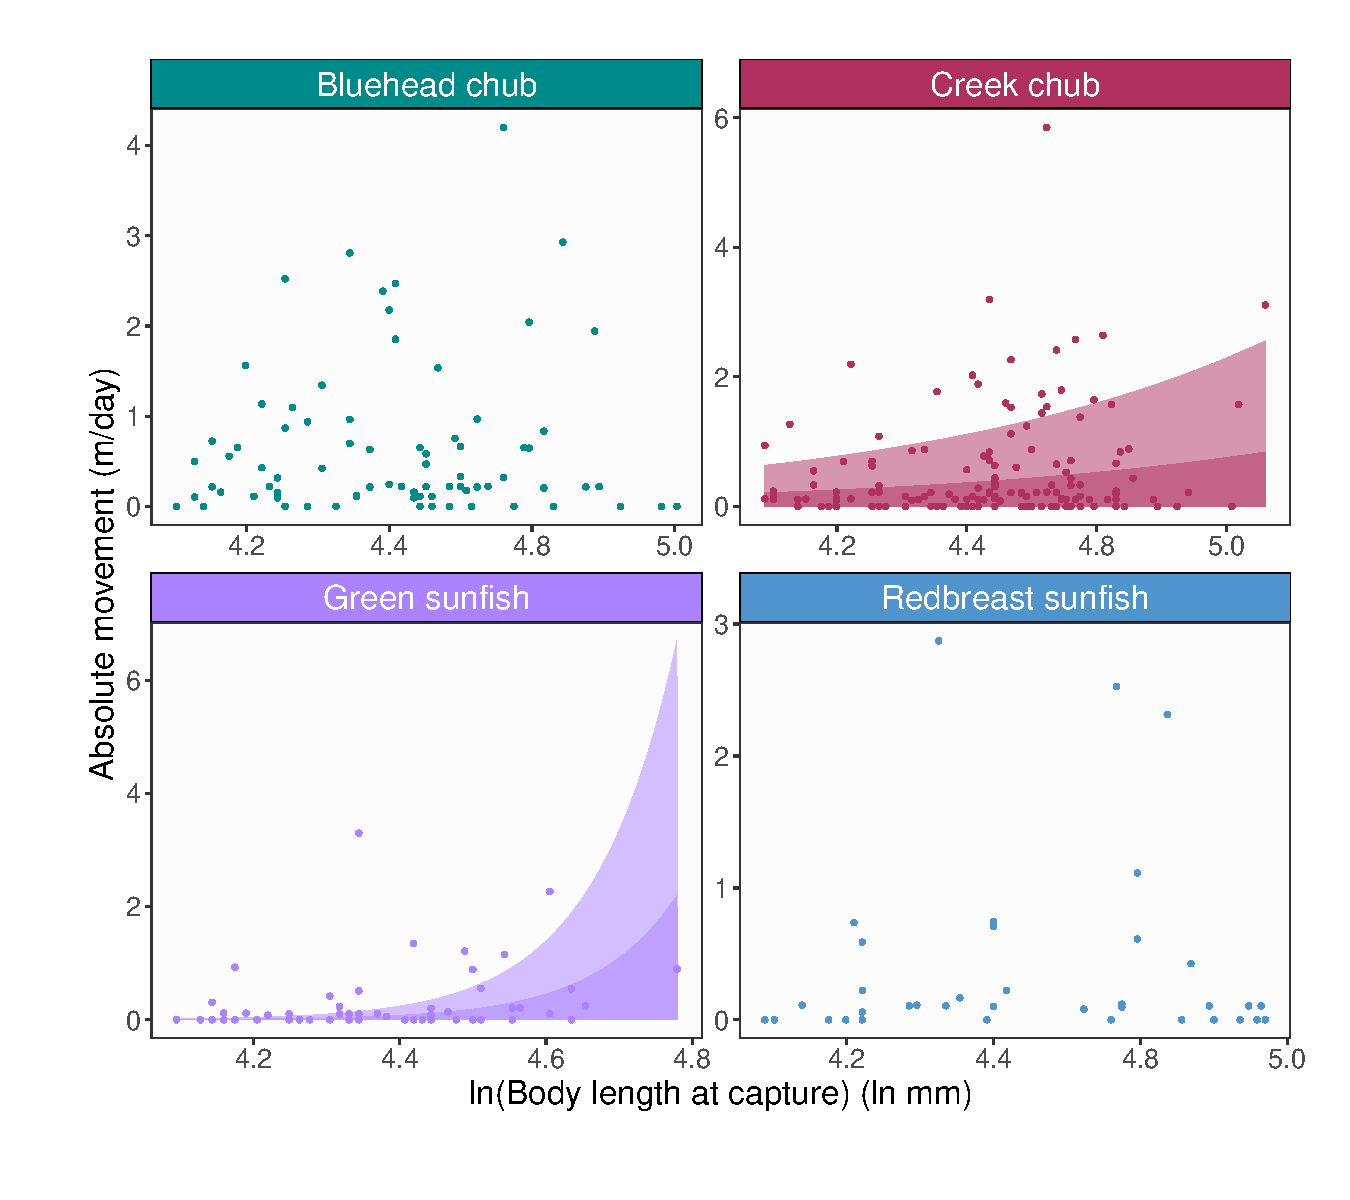
\includegraphics[width=0.75\linewidth]{output/fig_size.pdf}
    \caption{Influence of body size (total body length at capture) on movement distance. Panels and colors distinguish species. Points represent observed values for each recaptured individual. Dark and light shades indicate movement ranges that are predicted to encompass 50\% and 90\% of individuals by the observation-dispersal model. Shades are not shown when the posterior probability of the body size effect was less than 0.95. Full parameter estimates are provided in Table S5.}
    \label{fig:fig_size}
\end{figure}

Interspecific density-dependence in movement was observed in green and redbreast sunfish. Posterior distributions indicated that both species responded positively to the density of creek chub (Figures \ref{fig:fig_est} and \ref{fig:fig_density}), suggesting that these species moved away from areas with high population density of creek chub. 
In contrast, they tended to stay in areas with high population density of bluehead chub (Figure \ref{fig:fig_est}).
Bluehead chub and creek chub showed vague responses to other species' densities, although creek chub showed a marginal response to the densities of bluehead chub and green sunfish.
Interestingly, no species showed strong evidence of intraspecific density dependence in movement (Figure \ref{fig:fig_est}).

\begin{figure}
    \centering
    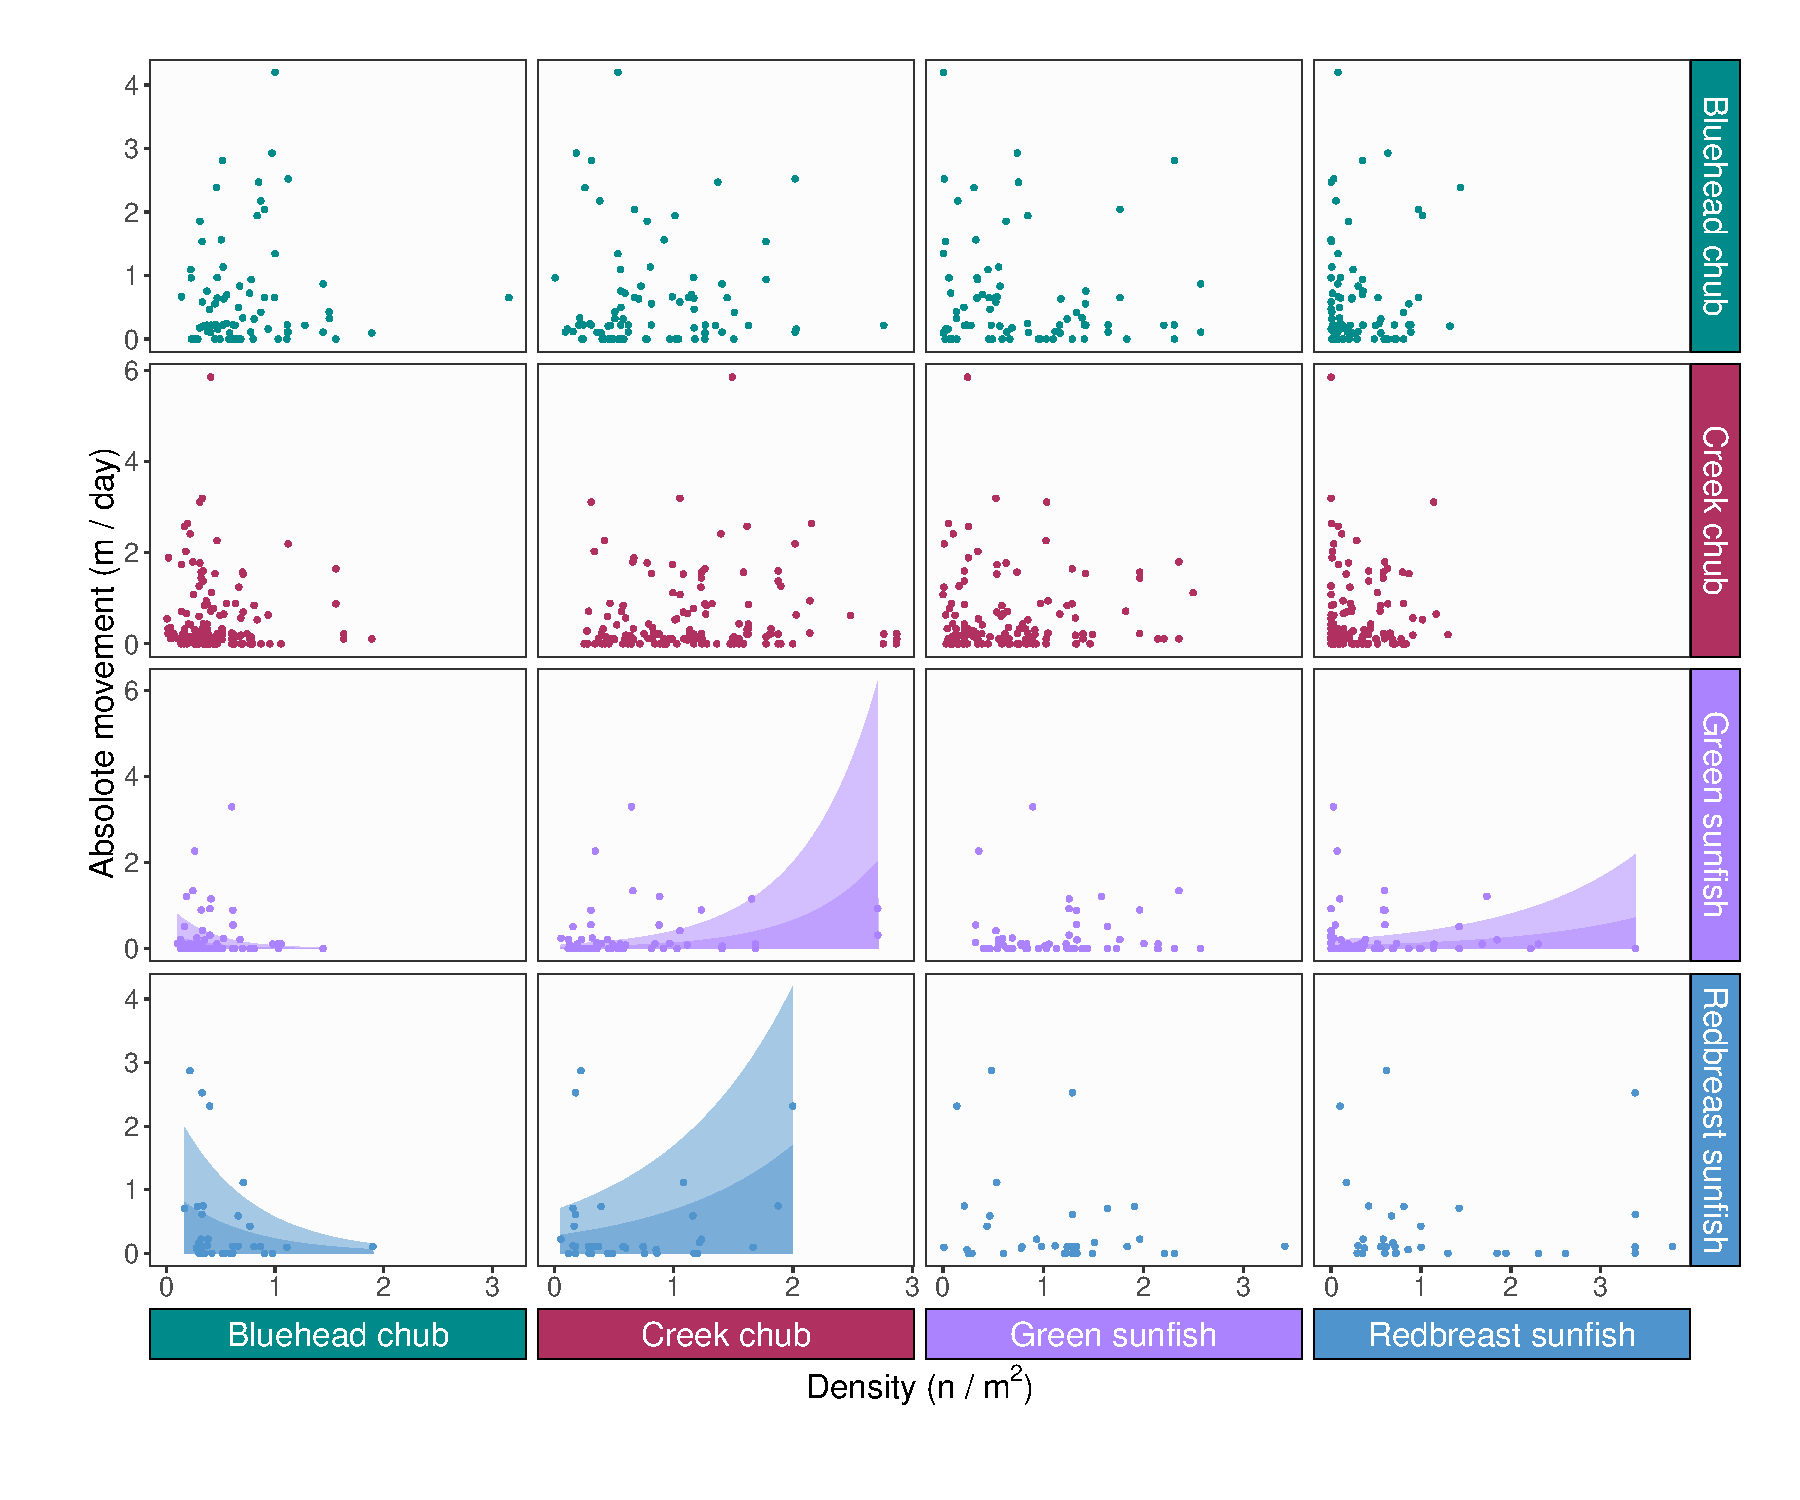
\includegraphics[width=0.8\linewidth]{output/fig_density.pdf}
    \caption{Influence of density on movement distance. Rows represent species responding to intra- and interspecific densities, while columns indicate the species whose population densities influence movement. Each panel describes the absolute movement of a species in response to the density of a given species. Colors represent response species. Diagonal panels show the response to intraspecific density, while the off-diagonal panels indicate the response to interspecific densities. Points represent observed values for each recaptured individual. Dark and light shades indicate movement ranges that are predicted to encompass 50\% and 90\% of individuals by the observation-dispersal model. Shades are not shown when the posterior probability of the density effect was less than 0.95. Full statistics are provided in Table S5.}
    \label{fig:fig_density}
\end{figure}

Green and redbreast sunfish reduced their movement in response to increasing HRA. Neither bluehead chub nor creek chub was influenced by HRA. The effect of current velocity was evident only for redbreast sunfish, which exhibited reduced movement distances in areas with swift currents. Temperature had a noticeable effect only on bluehead chub, which showed reduced movement during warmer periods. These results were summarized in  Table S5.

\section{Discussion}

Movement is shaped by species responses to extrinsic and intrinsic drivers \citep{clobertDispersalEcologyEvolution2012}. Yet, these factors are often studied in isolation, causing a lack of quantitative analysis comparing their relative influences. Our four-year data set of mark-recapture research unveiled that both intrinsic (body size) and extrinsic (population densities) factors influence stream fish movements, but their influences varied among species. While this makes our findings difficult to generalize, species-level movement responses can provide greater insight into how species interactions are distributed through non-random movement. 

Our first prediction of size-dependent movement was supported by creek chub and green sunfish. Movement requires great energetic expenditure that needs to be balanced among an individual’s needs \citep{boisclairImportanceActivityBioenergetics1989, joblingBioenergeticsFeedIntake1993, cookeMovementEcologyFishes2022}. Body size is one such limiting factor in determining metabolism \citep{beamish2SwimmingCapacity1978, rubio-graciaSizerelatedEffectsInfluence2020}. Because larger individuals have lower relative maintenance costs than smaller individuals due to greater lipid reserves \citep{brownSizeMattersTest2004, krauseRefugeUseFish1998, kannoBodyConditionMetrics2023}, they may be better able to balance the cost of moving \citep{schlagelMovementmediatedCommunityAssembly2020}. Not only are larger individuals at an energetic advantage, but they may serve as a stronger competitor in the settlement phase \citep{rasmussenIndividualMovementStream2017}. 
However, size-dependent movement patterns can be highly flexible and system-specific. For example, in South Carolina streams, creek chub did not exhibit size-dependent movement, whereas bluehead chub -- despite showing no such pattern in the present study -- demonstrated increased movement distance with body size \citep{teruiNonrandomDispersalSympatric2021}. Therefore, species that showed weak or no relationship between movement and body size in this study (bluehead chub and redbreast sunfish) might still exhibit size-dependent movement in other stream systems.
Comparative studies across multiple stream systems may offer deeper insights into the conditions under which size-dependence emerges.

Our second prediction -- higher interspecific density drives more movement -- was partially supported by green and redbreast sunfish, which moved longer distances as the density of creek chub increased. 
This positive interspecific density-dependence may be indicative of competition between species.
In small streams, like the one utilized here, the diets of our target species are known to overlap significantly \citep{collarPISCIVORYLIMITSDIVERSIFICATION2009, lemlySuppressionNativeFish1985, karrAssessmentBioticIntegrity1981, leonardApplicationTestingIndex1986}, potentially explaining the mechanism behind our observation.  
As a consequence of this movement process, sunfish species may move to potentially suboptimal habitats in order to avoid this type of interaction \citep{jacobHabitatChoiceMeets2018, thierryInterplayAbioticBiotic2024}. 
The green sunfish in particular may be successful in this approach as they are a hardy species that colonizes new areas well \citep{lemlySuppressionNativeFish1985, moyleInlandFishesCalifornia2002}.
However, creek chub did not move away from areas with a higher density of sunfish species, suggesting that this interspecific interaction through movement is asymmetric.
This result implies, albeit preliminarily, that creek chub is competitively superior to green and redbreast sunfish in our study stream.

Contrary to our expectations, however, these sunfish species tended to stay in areas with high bluehead density.
The exact mechanism is unclear, but predator-prey interactions might underlie this interspecific density-dependence \citep{jacobHabitatMatchingSpatial2015}. Green and redbreast sunfish have been documented to prey upon various chub species, including bluehead chub \citep{lemlySuppressionNativeFish1985, borrelliPuttingLakeTogether2023}.
In particular, small individuals of bluehead chub may be susceptible to predation by sunfish species. 
Thus, a higher density of bluehead chub may indicate greater food availability, potentially discouraging movement of these sunfish species.
Alternatively, shared environmental cues between the species, such as greater microhabitat (undercut bank, wood debris) availability, could explain a decrease in movement because these areas provide added refugia \citep{careyEffectsLittoralHabitat2010}.
While we cannot rule out the possibility of shared environmental cues, this mechanism is unlikely because the effects of microhabitat availability were statistically controlled in our model. Although experimental approaches are needed to elucidate biological causality, the trophic mechanism is more likely in our study system. 

% Bluehead chub and creek chub showed unclear responses to interspecific population density. The only exception was the decreased movement of creek chub in areas with higher redbreast sunfish density. Similar to the story above, predator-prey interactions may explain this observed pattern. Creek chubs are known omnivores feeding on a variety of insects, detritus, and fish \citep{champagneRiparianBuffersMaintain2022, leonardApplicationTestingIndex1986, quistSummerFoodHabits2006}. While there is no direct evidence for creek chubs predating upon redbreast sunfish, it is conceivable that larger creek chubs feed on smaller redbreast sunfish given the omnivorous nature of creek chubs.

Interestingly, no species responded significantly to intraspecific densities, countering our third prediction. This result is somewhat surprising given the wealth of studies showing intraspecific competition exceeding interspecific competition in fishes \citep{websterMechanismsIndividualConsequences2000, wardIntraspecificFoodCompetition2006} and other taxa \citep{adlerCompetitionCoexistencePlant2018, barabasEffectIntraInterspecific2016, thompsonProcessbasedMetacommunityFramework2020, chessonRolesHarshFluctuating1997, tilmanResourceCompetitionCommunity1982, mcpeekIntraspecificDensityDependence2012}. While high conspecific density could impose intensive intraspecific competition, it also increases the likelihood of finding potential mates, dilution effects, and group feeding (e.g., Allee effects) \citep{courchampAlleeEffectsEcology2008, gascoigneAlleeEffectsDriven2004, teruiCrypticAlleeEffect2015}. In our system, this may overshadow the relative competition for other resources like habitat and food, thus producing stronger interspecific interactions. Although further studies are needed to illuminate underlying mechanisms, these opposing influences of conspecific density could potentially obscure the influence on movement patterns. 

Although our study illuminated interesting patterns, the results must be viewed with caution. First, while we selected extrinsic and intrinsic variables representative of individual movement ability and species interactions, other potential variables (e.g., sex, disturbance) may be playing a role in driving movement.
Evaluating movement as it occurs \textit{in situ} is an ambitious task; as a consequence, not all possible drivers of movement could be evaluated, like any other field study.
This limitation could explain why one of the study species, bluhead chub, did not show clear movement patterns in response to selected intrinsic and extrinsic variables.
Combining field research with controlled experiments may help address this limitation \citep{fronhoferBottomupTopdownControl2018, nathanMovementEcologyParadigm2008}.
Second, we experienced relatively low consecutive recapture rates, likely because of the small spatial extent of our study area. Our dispersal-observation model is best suited for this type of data though, as it accounts for emigration from the 430-m study reach, imperfect detection, and survival processes to minimize statistical biases arising from this limitation \citep{teruiModelingDispersalUsing2020}.
Our simulation study found that this modeling approach provides unbiased estimates of movement parameters, even if the proportion of recaptures is $\sim$0.25.
Yet, low recapture rates increase the uncertainty of parameter estimates \citep{teruiModelingDispersalUsing2020}.
Although our results should be qualitatively robust, their effect size must be interpreted carefully.
Lastly, we observed ``outlier'' movers in the data (Figures \ref{fig:fig_size} and \ref{fig:fig_density}). 
However, since our model employed a Student-t distribution (see Equation \ref{eq:student-t}), our statistical inference is insensitive to these outlier values (i.e., conservative) \citep{lunnBUGSBookPractical2012}. 
Nevertheless, it is important to recognize that long-distance movers can play critical roles in ecological processes \citep{clobertDispersalEcologyEvolution2012}.
Future studies addressing this limitation would be particularly valuable in advancing movement research.

Movement mediates how species interact, shaping the dynamics of spatially-structured communities \citep{schlagelMovementmediatedCommunityAssembly2020}. Our study demonstrates how intrinsic (e.g., body size) and extrinsic (e.g., population density) drivers can help pinpoint potential movement patterns in freshwater fishes, with variation among species elucidating a potential avenue to explore community dynamics in the future. Extrapolating how non-random movements, such as those identified in this study, affect species coexistence and the spatial patterns of community organization will be essential in connecting behavioral ecology to spatial theory.

\bibliography{tex/references}

\newpage

\section*{Data Accessibility}
All data and R code can be found on the GitHub repository under the following link: \url{https://github.com/ashleylaroque/public_cmr_movement}

\section*{Competing Interests}

None declared.

\section*{Author Contributions}

A.T. and A.L. conceived the idea; A.L., S.K., and A.T. performed  field work; A.L. and A.T. performed statistical analysis and drafted the manuscript; All authors contributed to revision and gave final approval for  publication.

\section*{Acknowledgments}

This work is based on materials supported by University of North Carolina at Greensboro Startup, the Faculty Internal Award, John O'Brien Ecological Field Award, and Dorothy Levis Munroe Research Award funds. We graciously thank our undergraduate students for their help in conducting seasonal fieldwork and digitizing data. We are grateful to University of North Carolina at Greensboro and North Carolina Agricultural and Technical State University for their corroboration in granting us access to Gateway Research Park. 


\end{document}